%%%%%%%%%%%%%%%%%%%%%%%%%%%%%%%%%%%%%%%%%%%%%%%%%%%%%%%%%%%%%%%%%%%%%%%%%%%%%%%

\documentclass[12pt,twocolumn,tighten]{aastex62}
%\documentclass[12pt,twocolumn,tighten,trackchanges]{aastex62}
\usepackage{amsmath,amstext,amssymb}
\usepackage[T1]{fontenc}
\usepackage{apjfonts}
\usepackage[figure,figure*]{hypcap}
\usepackage{graphics,graphicx}
\usepackage{hyperref}
\usepackage{natbib}

\renewcommand*{\sectionautorefname}{Section} %for \autoref
\renewcommand*{\subsectionautorefname}{Section} %for \autoref

\newcommand{\ptfo}{PTFO$\,$8-8695}
\newcommand{\ptfob}{PTFO$\,$8-8695b}

%% Reintroduced the \received and \accepted commands from AASTeX v5.2.
%% Add "Submitted to " argument.
\received{\today}
\revised{---}
\accepted{---}
\submitjournal{AAS journals.}
\shorttitle{Seeing Double: PTFO$\,$8-8695}

\begin{document}

\defcitealias{bouma_wasp4b_2019}{B19}

%\title{Against the Planetary Interpretation of PTFO$\,$8-8695b}
% \title{Seeing Double: Still Against the Planetary Interpretation of
% PTFO$\,$8-8695b}
% \title{Seeing Double: TESS and Gaia Show That PTFO$\,$8-8695b is Unlikely a
% Planet}
\title{Seeing Double: Indications From {\it TESS} and {\it Gaia} That
PTFO$\,$8-8695b is Not a Planet}

\correspondingauthor{L. G. Bouma}
\email{luke@astro.princeton.edu}

%
% key authors:
%
\author[0000-0002-0514-5538]{L. G. Bouma}
\affiliation{ Department of Astrophysical Sciences, Princeton
University, 4 Ivy Lane, Princeton, NJ 08540, USA}
%
\author[0000-0002-4265-047X]{J. N. Winn}
\affiliation{ Department of Astrophysical Sciences, Princeton
University, 4 Ivy Lane, Princeton, NJ 08540, USA}

\begin{abstract}
  PTFO$\,$8-8695b is a candidate hot Jupiter in the 7--10 million year old
  Orion-OB1a cluster. We inspected data from TESS and Gaia to clarify whether
  it is actually a planet.  The TESS lightcurve shows that the dominant
  variability in this system is a sinusoid with a ``long'' period $P_{\rm
  \ell}=11.96\,$hr, likely caused by stellar rotation.  Also present is a
  complex signal, previously identified as the planet candidate, that repeats
  with a ``short'' period $P_{\rm s}= 10.74\,$hr.  The two signals beat every
  4.48 days.  Although there is a dip in the short-period signal, ground-based
  photometry from the past decade shows that the orbital phase of the dip seems
  to have instantaneously jumped, at least once, and perhaps twice.  Planets do
  not ``jump'' in orbital phase.  Furthermore, the Gaia data show that
  PTFO$\,$8-8695 is probably a photometric binary.  Given the evidence, we
  believe that PTFO$\,$8-8695 is a binary M dwarf in which one star shows the
  ``long'' rotation signal, and the other is showing ``transient dipping'' that
  has also been observed in other young M dwarfs.  The planetary interpretation
  seems unlikely.
\end{abstract}

%TODO
\keywords{
	Exoplanet evolution (491),
	Open star clusters (1160),
	Stellar ages (1581),
	Stellar rotation (1629),
	Variable stars (1761)
}

%%%%%%%%%%%%%%%%%%%%%%%%%%%%%%%%%%%%%%%%%%%%%%%%%%%%%%%%%%%%%%%%%%%%%%%%%%%%%%%

\section{Introduction}
If \ptfob\ were a planet, it would be exceptional.  Transiting a sub-10$\,$Myr
old weak-lined T Tauri M dwarf in Orion, it would be the youngest hot Jupiter
known \citep{van_eyken_ptf_2012}.  Its orbital period of only 10.7 hours would
also give it the shortest period of any known hot Jupiter.  With such a short
period, it would almost certainly have filled its Roche lobe, and would be
actively losing mass to its host star.  Not only that, but the rapidly rotating
host star would also be oblate and gravity darkened, and so the planet's orbit
would likely precess into and out of transitability
\citep{barnes_measurement_2013,ciardi_followup_2015,kamiaka_revisiting_2015}. 

Other lines of evidence would imply further planetary ``firsts'' for
this planet candidate.  One first would be that its transits are about three
times deeper in optical bandpasses ({\it e.g.,} $g$-band) than in the near-infrared
({\it e.g.}, $z$-band) \citep{onitsuka_multicolor_2017,tanimoto_evidence_2020}.
A cloud-free hydrogen-dominated planetary atmosphere cannot explain such a
wavelength dependence.  The planet might therefore be surrounded by a
dust cloud \citep{tanimoto_evidence_2020}.  

Another first could be the direct detection of H$\alpha$ emission from the
planet itself \citep{johnskrull_h_2016}.  While the stellar chromosphere emits
in H$\alpha$, it seems that there is an additional excess H$\alpha$ emission
that could be in phase with the planetary orbit.  The average velocity width of
the excess H$\alpha$ emission is 87$\,$km$\,$s$^{-1}$, and its equivalent width
is 70-80\% that of the stellar chromosphere \citep{johnskrull_h_2016}.  The
proposed explanation is that the outflowing mass from the planet may explain
this excess emission as well \citep{johnskrull_h_2016}.

There are perhaps a few challenges to the planetary interpretation (if
these ``features'' are not already seen as such).  They include that
the planet does not seem to emit infrared radiation in occulation, at
least anywhere near the expected amplitude \citep{yu_tests_2015}.  In
addition, despite measurement attempts by multiple investigators, it
does not seem to show the Rossiter effect at the amplitude expected
given the rapid stellar rotation and large planet size
\citep{yu_tests_2015,ciardi_followup_2015}.  Finally, detailed
modelling of the ``precession + gravity darkening'' transits has shown
that the necessary degree of gravity darkening is too great, given the
spectroscopically observed equatorial velocity
\citep{howarth_reappraisal_2016}.  Additionally, as the gravity-darkened
star precessed about its rotation axis, it would need to show
photometric variability that has not been observed.

While the planetary interpetation has challenges, alternative
explanations do as well.  High-latitude accretion hotspots might
produce the observed H$\alpha$ variability, but \ptfo\ does not have
an infrared (IR) excess associated with the presence of an inner disk.
Low-latitude starspots, hot or cold, struggle to produce the necessary
dip durations.  A circumstellar cloud of dust or gas might be
entrained in the stellar magnetosphere, but clumps would need to be
invoked to explain the short-duration flux dips. 

In the following, Section~\ref{sec:observations} presents newly
available observations from the Transiting Exoplanet Survey Satellite
(TESS; \citealt{ricker_transiting_2015}) and Gaia
\citep{gaia_collaboration_gaia_2018}.  Analyzing the TESS data in
Section~\ref{sec:tess}, we find two distinct signals.  A long sinusoid
repeats every 12.0 hours, and is probably stellar rotation.  A short
``dip + complex modulation'' repeats every 10.7 hours.  Analyzing the
Gaia data in Section~\ref{sec:gaia}, we show that \ptfo\ is quite
likely a photometric binary.  In Section~\ref{sec:discussion}, we note
that the orbital phase of the dip seems to have instantaneously
changed, perhaps twice.  We argue that PTFO$\,$8-8695 is a binary M
dwarf in which one star shows a rotation signal, and the other is
showing ``transient dipping'' that has been observed in other young M
dwarfs, and is likely caused by eclipses of warm particulate clouds.
Section~\ref{sec:conclusions} summarizes our main points.


\section{The Data}
\label{sec:observations}

\begin{figure*}[t!]
	\begin{center}
		\leavevmode
		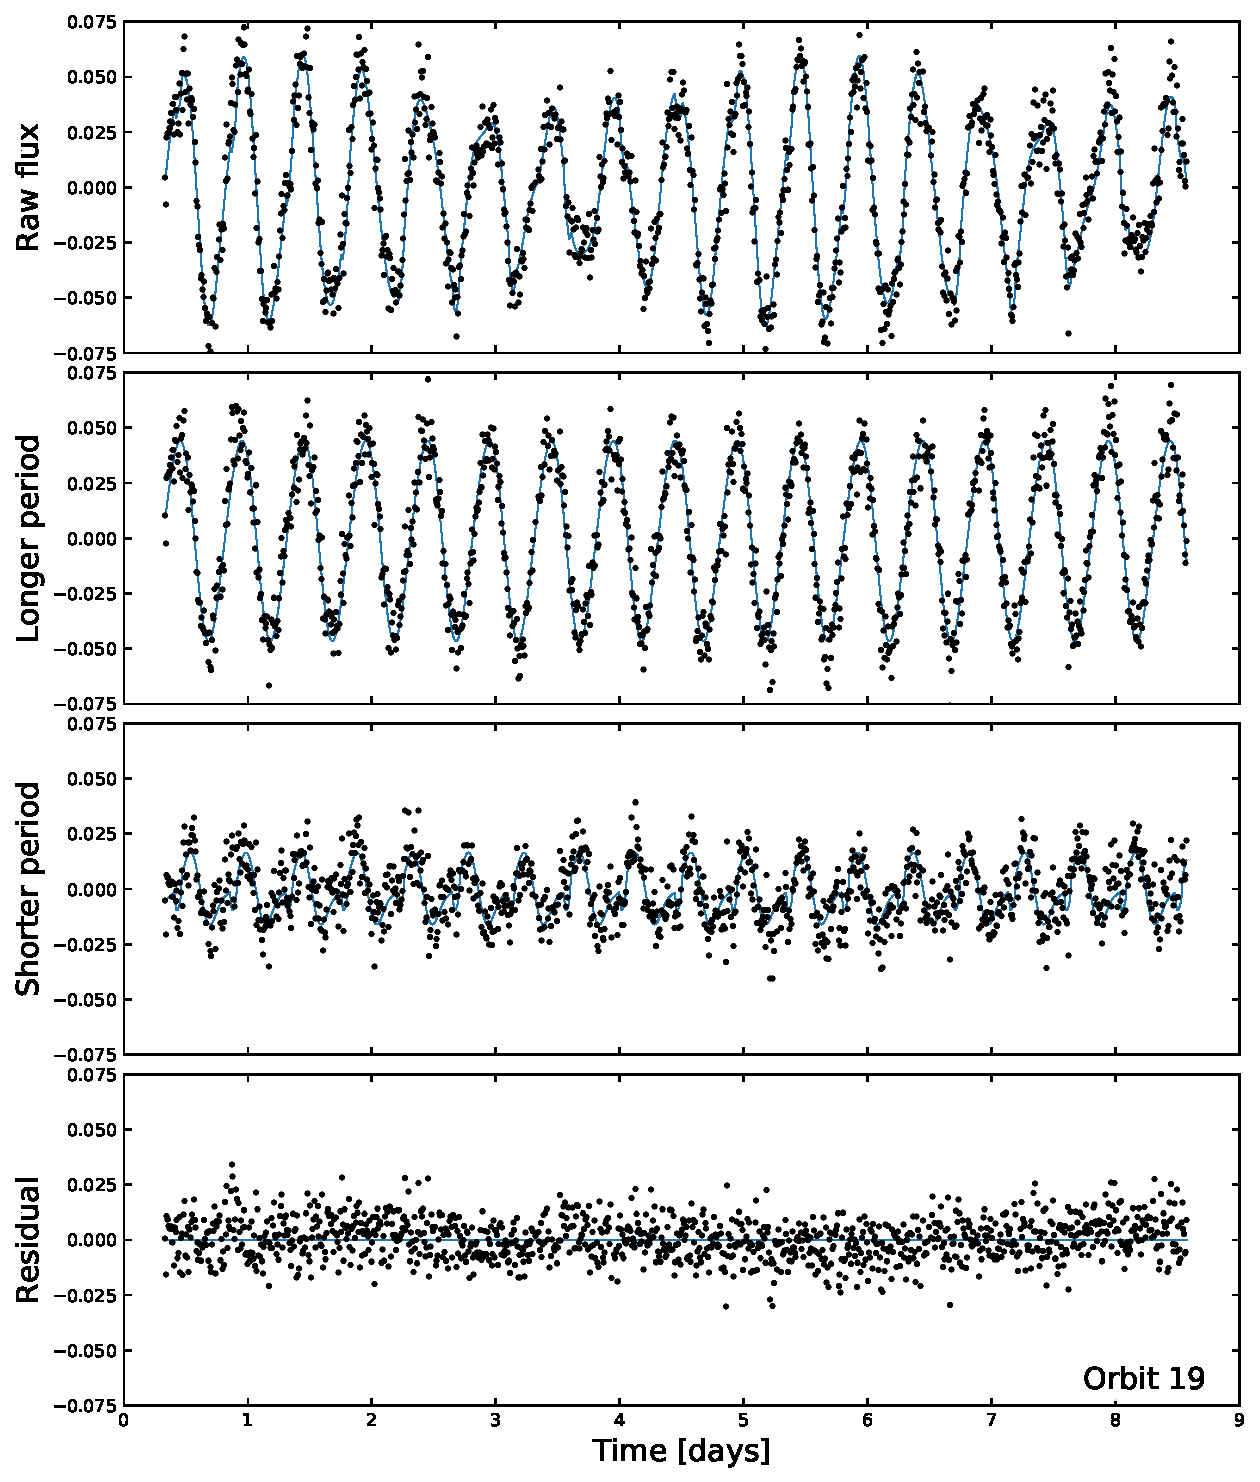
\includegraphics[width=1\textwidth]{f1.pdf}
	\end{center}
	\vspace{-0.7cm}
	\caption{
		{\bf TESS lightcurve of \ptfo\ (Sector 6, Orbit 19).}
		{\it Top}: ``Raw'' \texttt{PDCSAP} mean-subtracted relative flux
		versus time. The beat period of 4.48 days is visible by eye.  The
		preferred model plotted underneath the data includes 2 harmonics at the long
		period $P_{\rm \ell}$, plus 2 harmonics and a transit at the short
		period $P_{\rm s}$.
		{\it Upper middle}: Long-period signal, equal to the raw signal
		minus the short-period signal.
		{\it Lower middle}: Short-period signal, equal to the raw signal
		minus the long-period signal.
		{\it Bottom}: residual.  The data are binned from 2 to 10 minute
		cadence as a convenience for plotting and fitting.
		\label{fig:splitsignal}
	}
\end{figure*}

\begin{figure*}[hbtp]
	\begin{center}
		\leavevmode
		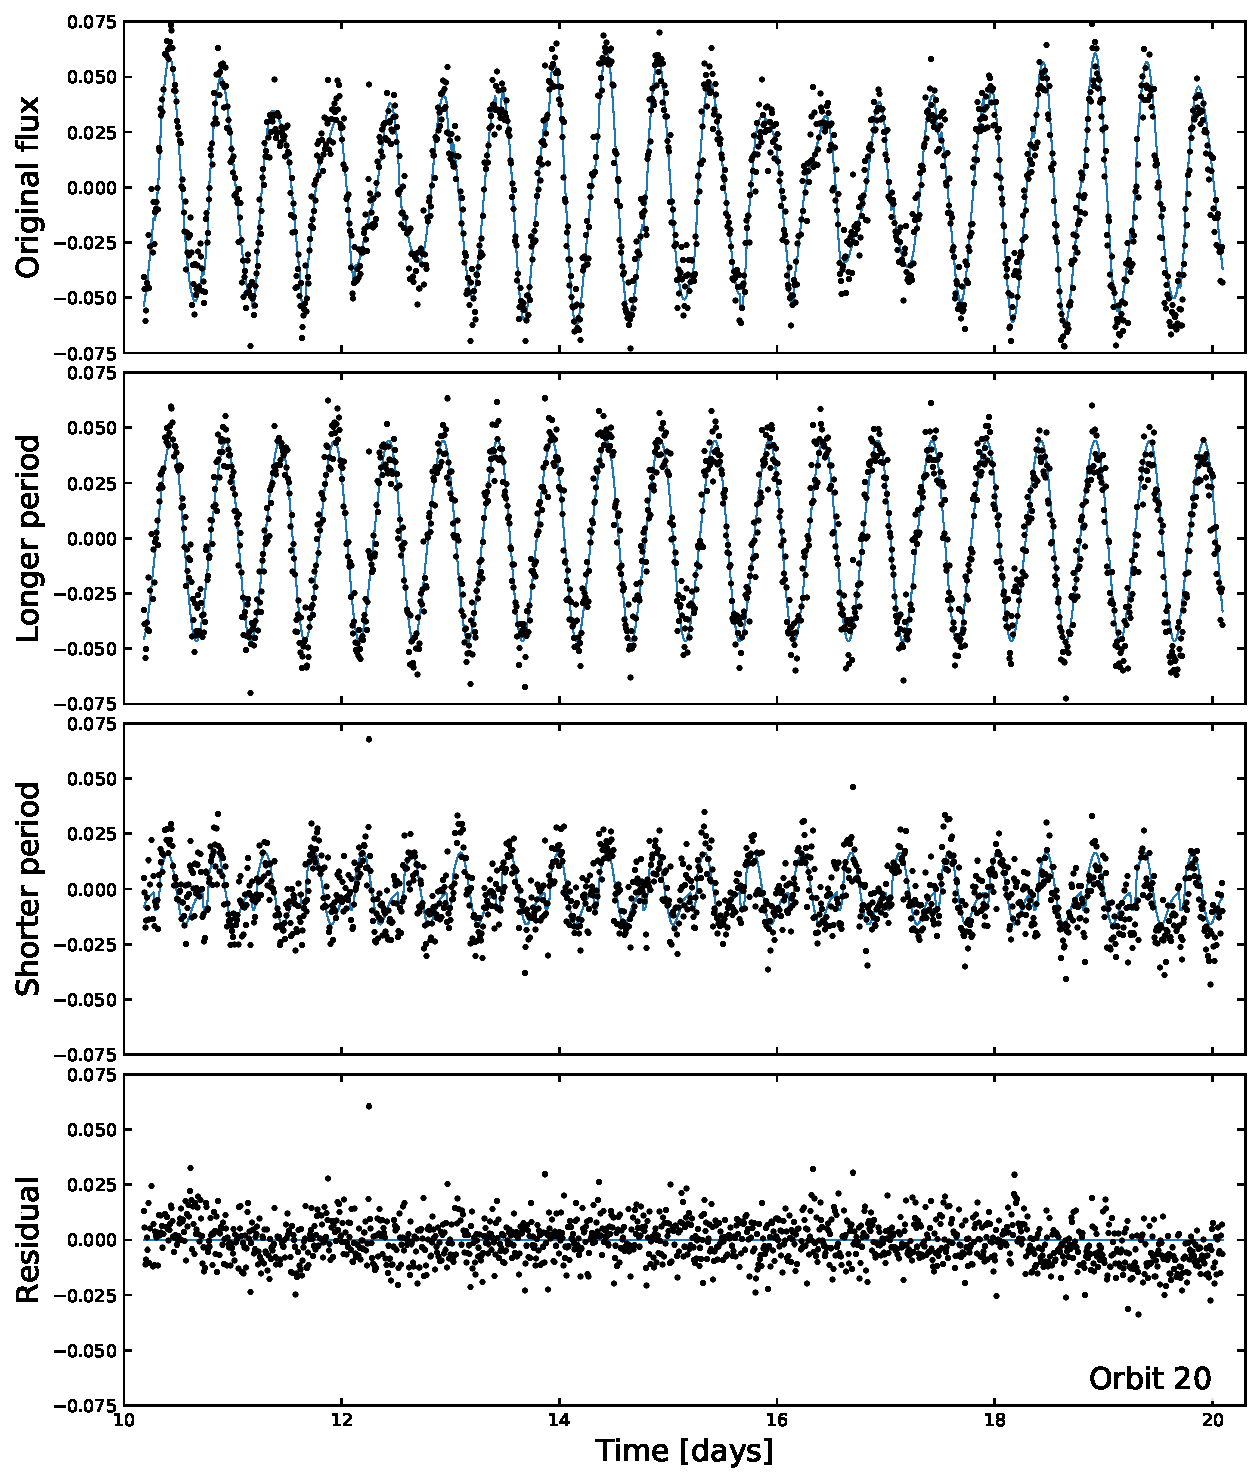
\includegraphics[width=1\textwidth]{f2.pdf}
	\end{center}
	\vspace{-0.7cm}
  \caption{ {\bf TESS lightcurve of \ptfo\ (Sector 6, Orbit 20).}
		Panels are as in Figure~\ref{fig:splitsignal}.
		\label{fig:splitsignalii}
	}
\end{figure*}


%\begin{figure*}[t!]
%	\begin{center}
%		\leavevmode
%		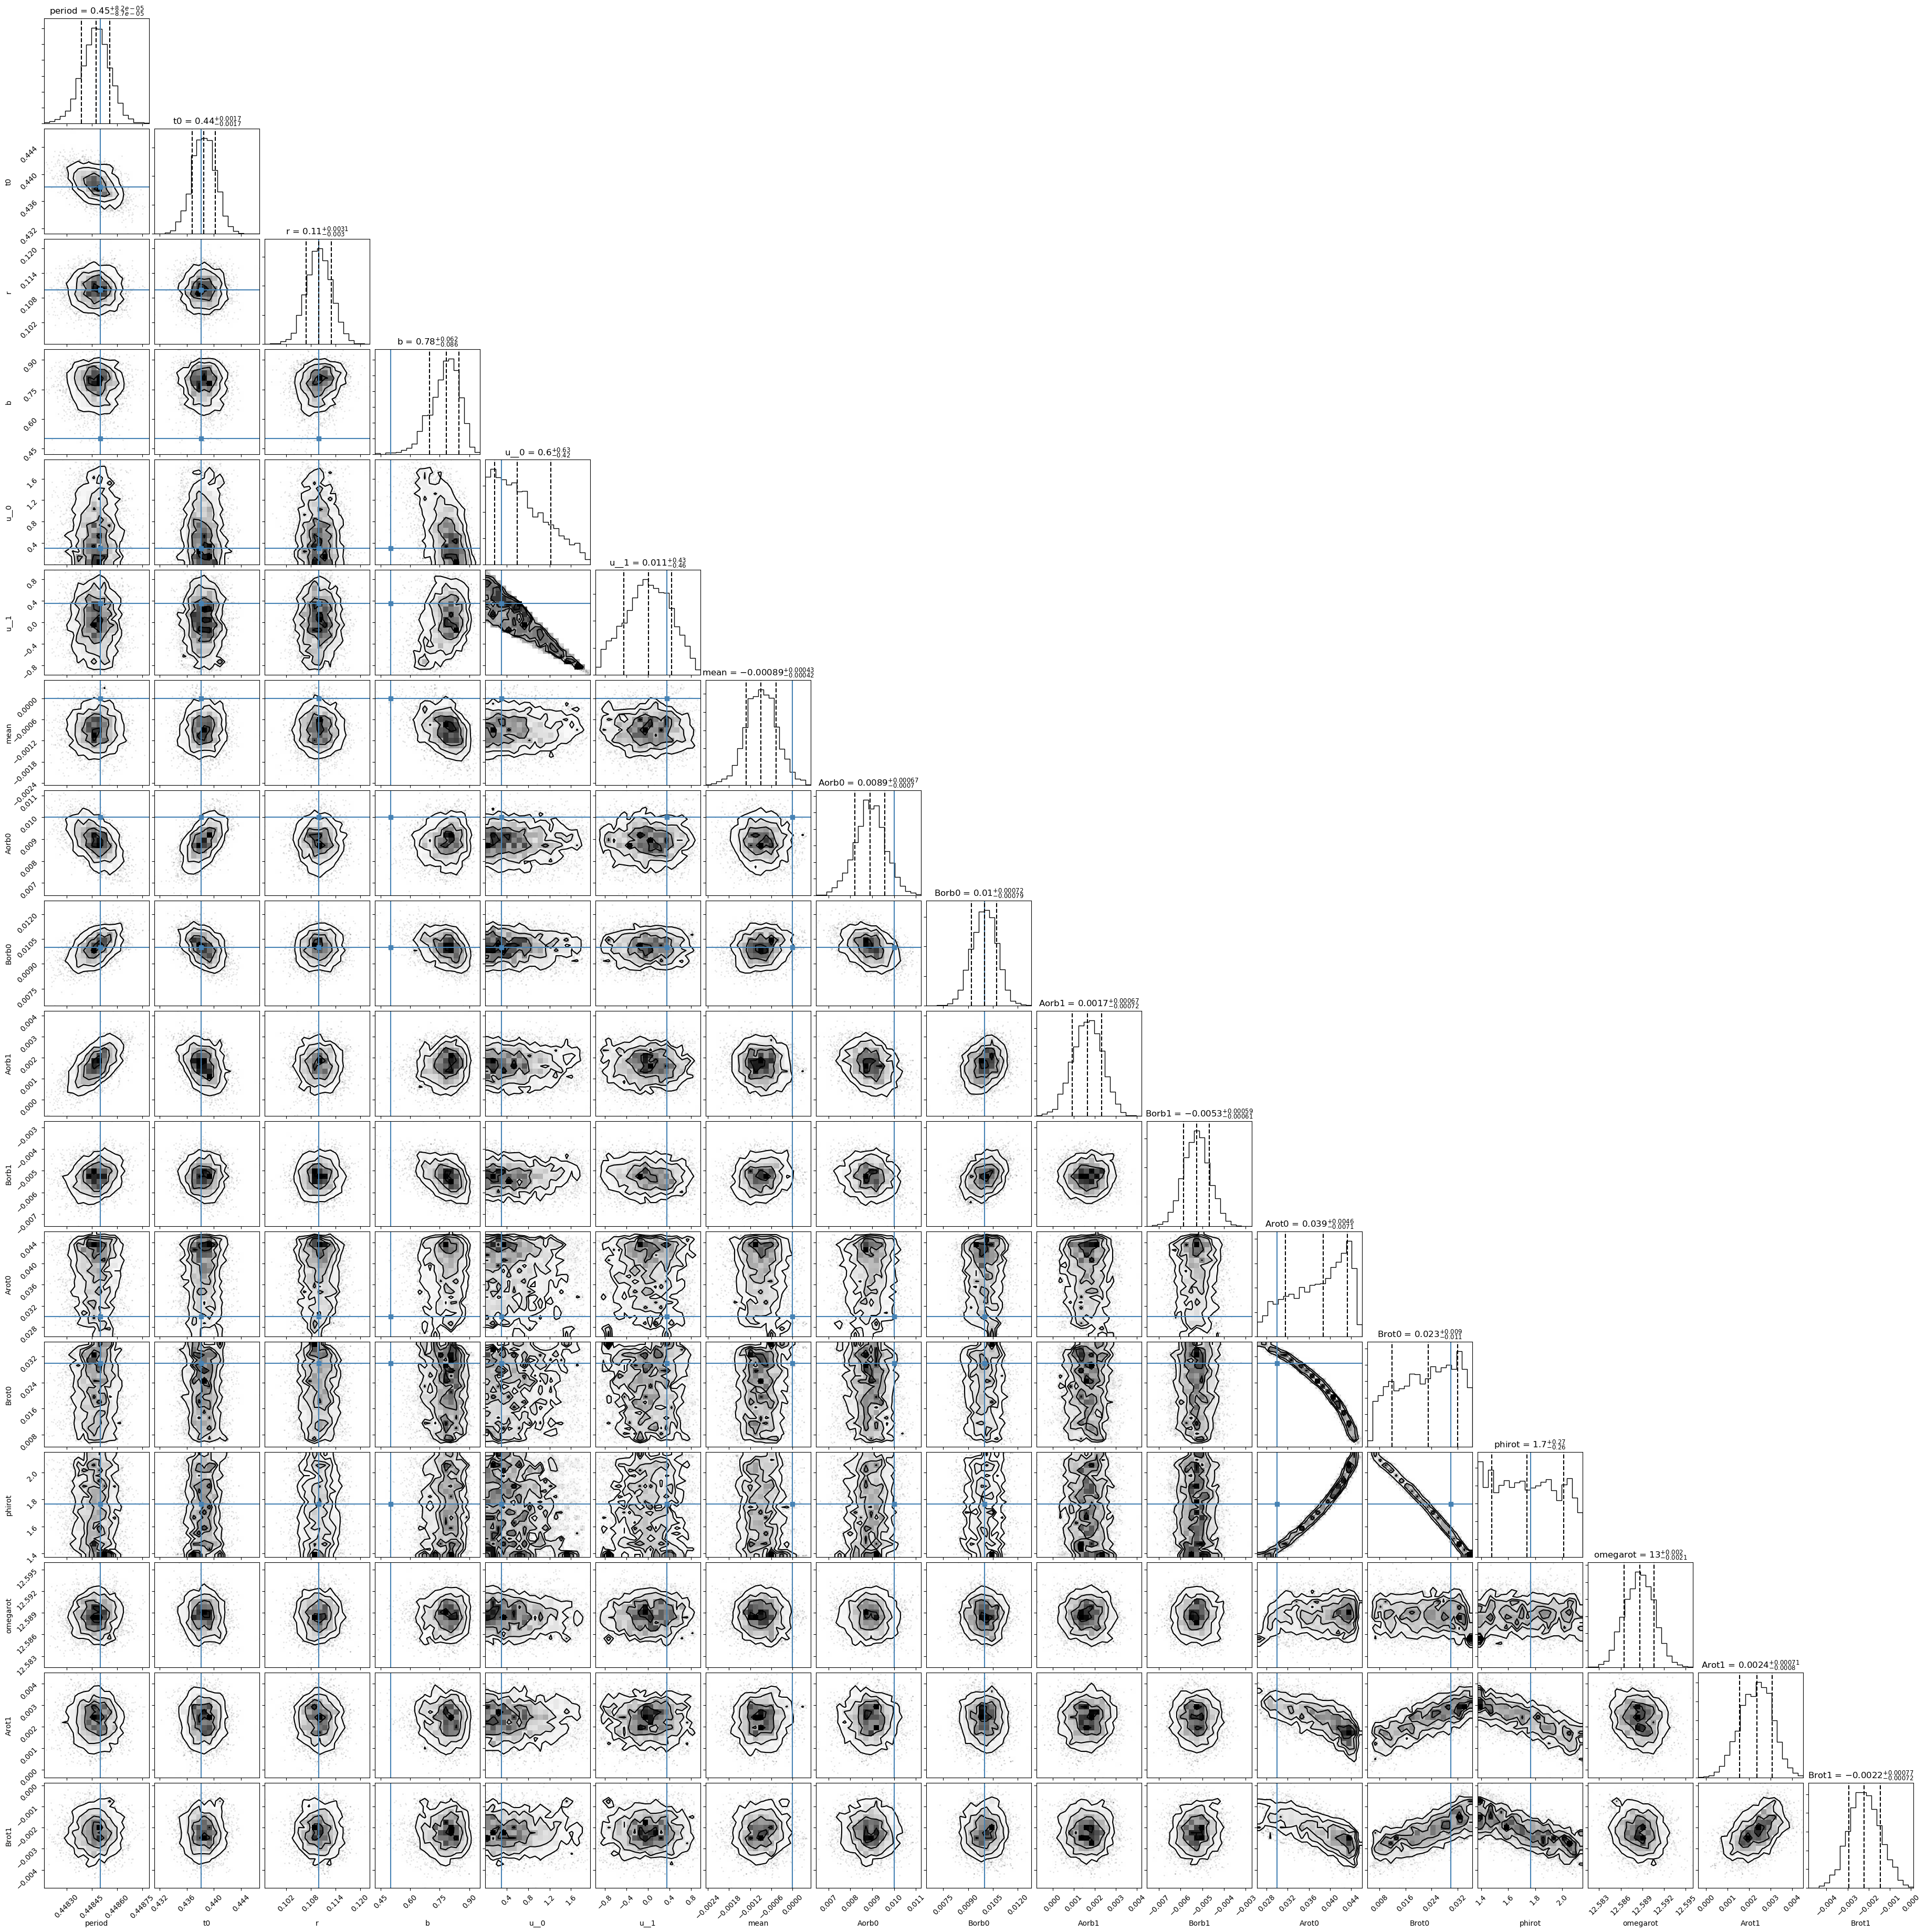
\includegraphics[width=0.9\textwidth]{f6_comp.png}
%	\end{center}
%	\vspace{-0.7cm}
%	\caption{ {\bf foo.}
%	bar
%		\label{fig:corner}
%	}
%\end{figure*}

\subsection{TESS Observations}

\ptfo\ was observed by TESS with Camera 1, CCD 1, from December
15, 2018 to January 6, 2019, during the sixth sector of science
operations \citep{ricker_transiting_2015}.  The star was designated
TIC 264461976 in the TESS Input Catalog
\citep{stassun_TIC_2018,stassun_TIC8_2019}.  The pixel data for an
$11\times11$ array surrounding \ptfo\ were averaged into 2-minute
stacks by the onboard computer.  Each 2048$\times$2048 image from the
CCD was also averaged into 30-minute stacks, and saved as a ``full
frame image'' (FFI).

The 2-minute stacks for \ptfo\ were then reduced to lightcurves
by the Science Processing Operations Center (SPOC) at NASA
Ames~\citep{jenkins_tess_2016}.  Our main analysis used the resulting
Presearch Data Conditioning (PDC) lightcurve.  The PDC lightcurve
aperture used pixels chosen to maximize the SNR of the total flux of
the target \citep{smith_kepler_apertures_2017}.  Non-astrophysical
variability was removed through the methods discussed by
\citet{smith_kepler_PDC_2017}.

As an independent check on the shorter cadence SPOC light-curve, we
separately processed the 30-minute image stacks as part of the Cluster
Difference Imaging Photometric Survey (CDIPS;
\citealt{bouma_cluster_2019}).  The CDIPS lightcurve used a circular
aperture with radius 1 pixel.

To clean the data, we removed all points with non-zero quality flags
\citep[{\it e.g.},][]{tess_data_product_description_2018}.  We also
masked out the first and last 6 hours of each orbit, since there is
often systematic red noise during those times.  Both the CDIPS and PDC
lightcurves showed a clear discontinuous ``jump'' in the last few days
of orbit 20, which seemed likely to be an instrumental systematic.  We
correspondingly masked out times from BJD 2458488.3 until the end of
the orbit.  The PDC lightcurve initially had 15{,}678 points.  The
quality cut removed 854 points, masking the orbit edges removed an
additional 716, and removing the final few days of orbit 20 removed an
additional 1079.  After cleaning, 83\% of the initial flux
measurements remained.

We normalized these points by dividing out the median flux. We then
subtracted by unity to simplify subsequent analysis.  Many of these
and subsequent processing steps were performed using
\texttt{astrobase}~\citep{bhatti_astrobase_2018}. 


\subsection{Gaia Observations}

Between July 25, 2014 and May 23, 2016, Gaia acquired 121 ``good''
observations of \ptfo, {\it i.e.}, observations that were not strongly
downweighted in the astrometric solution of the source (CITE).
%TODO: give an original explanation of how Gaia works
The Gaia data processing team at XXXINSTITUTION combined the XXX and
YYY into a global astrometric solution, from which the parallax of 
\ptfo\ was derived (CITE).
The star was assigned a Gaia DR2 identifier of 3222255959210123904
(CITE).
In addition, measurements of the stellar proper motion between
observation epochs were made.
%FIXME sentence is bad

One point of note:
Gaia DR2 measured a significant ``astrometric excess'', at a level of
10.3$\sigma$.
This astrometric excess indicates the degree
to which a single-source model fails to explain the observed astrometric
measurements (CITE).

\subsection{Cluster Membership}
The Orion molecular cloud complex has numerous subgroups, with ages
spanning 1 to 15$\,$Myr (CITE).
\ptfo\ has been known to be a member of the Orion OB1a association
since at least CITE (Briceno 2005).
Its relation to the broader Orion complex has been further explored by
CITEX, CITEY, and CITEZ (Briceno 05, 08, 18, whomever Van Eyken cites,
and Kounkel 18).

In describing the cluster membership of \ptfo, we follow the notation
and results of \citet{kounkel_apogee2_2018}.
\citet{kounkel_apogee2_2018} combined astrometric data from Gaia DR2
with spectroscopic data from APOGEE-2 (CITE).  They then performed a
hierarchical clustering on the six dimensional position and velocity
information to identify subgroups within the Orion complex.  From
smallest to largest groups, \ptfo\ was identified as being a member of
the following nested subgroups:
\begin{equation}
  %{\rm PTFO\,8\text{-}8695}
  % \in
  {\rm 25\,Ori\text{-}1}
  \subset {\rm 25\,Ori}
  \subset {\rm Orion\ OB1a}
  \subset {\rm Orion\ D},
\end{equation}
where from set-notation, `$\subset$' denotes ``is a proper subset of''.

While all members of the Orion complex are young relative to the
field, the internal age dispersion between different subgroups is
measurable.  The Orion Nebula Cluster (M42) is a site of ongoing
star-formation, and its stars are 1-3$\,$Myr old (CITE).
25$\,$Ori\-1, by contrast, is XX-XX$\,$Myr old (CITE).  These details
are essential when assessing any evidence for photometric binarity in
\ptfo, because there is a degeneracy between stellar luminosity and
age for stars on the pre-main-sequence.  Having a clean sample of
tightly spatially and kinematically associated stars is essential to
minimize contamination not just from the field, but from older and
younger members of the Orion complex itself.


\section{TESS Analysis}
\label{sec:tess}

\begin{figure*}[t]
	\begin{center}
		\leavevmode
		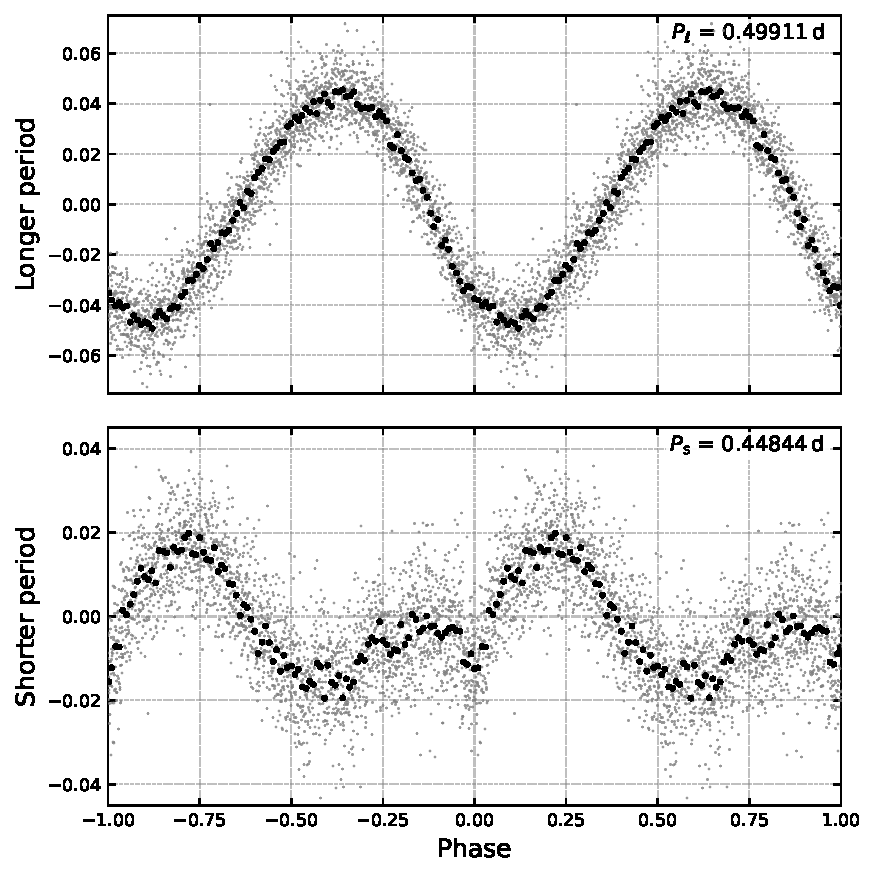
\includegraphics[width=0.99\textwidth]{f3.pdf}
	\end{center}
	\vspace{-0.7cm}
	\caption{ {\bf Phase-folded long and short-period signals.}
		{\it Top}: Long-period signal, as in Figure~\ref{fig:splitsignal}.
		{\it Bottom}: Short-period signal. The reference phase is set to the
		``planetary'' dip.  Gray points are the 10 minute cadence
		\texttt{PDCSAP} flux.  Black points are binned to 100 points per
		period.
		\label{fig:phasefold}
	}
\end{figure*}

\subsection{Inspection}

Our initial inspection of the lightcurve, in both its 2-minute PDCSAP
and 30-minute FFI forms, showed a strong sinusoidal beat signal
(Figure~\ref{fig:splitsignal}, top panel).

As a precursor to more detailed analysis, we calculated generalized
Lomb-Scargle periodograms using \texttt{astrobase}
\citep{lomb_1976,scargle_studies_1982,vanderplas_periodograms_2015,bhatti_astrobase_2018}.
The two largest peaks in the Lomb-Scargle periodogram of the
lightcurve were clearly separated at a ``short'' period $P_{\rm s}
\approx 0.448\,{\rm days}$ and a ``long'' period $P_{\rm \ell} \approx
0.499\,{\rm days}$.  The $P_{\rm \ell}$ peak had the greater power of
the two.  Smaller harmonics from each of these two dominants peaks
were also present.

% 0.14 = A1+A2
% 0.06 = A1-A2
% 2A1 = 0.20
% -> A1 = 0.1
% 2A2 = 0.08
% -> A2 = 0.04

The peak-to-peak amplitude at maximum, when the two signals
constructively interfere, is about 14\%.  At minimum, the peak-to-peak
amplitude is about 6\%.  Assuming the signals are just two sinusoids,
algebra tells us that the peak-to-peak amplitudes should therefore be
10\% for the long-period signal, and 4\% for the short-period signal.
These order-of-magnitude numbers will turn out to be roughly correct.

Initial signal-processing experiments fitting out splines or sinusoids
showed that after subtracting out the long-period signal, the
short-period signal dominated the periodogram, and vice-versa.
However it quickly became clear that it would be beneficial to
simultaneously model the signals separately, in order to preserve the
power at each frequency.




\subsection{Lightcurve Model}

We opted to model the lightcurve as a linear combination of Fourier
harmonics at the short and long periods, plus a transit at the short
period.  Symbolically, the total flux $f$ is given as
\begin{equation}
  f = f_{\rm s} + f_{\rm \ell}
  = f_{\rm transit,s} + f_{\rm Fourier,s} + f_{\rm Fourier,\ell},
\end{equation}
where $f_{\rm s}$ is the relative flux at the short period, and
$f_{\rm \ell}$ is the flux at the long period.  Writing out the
Fourier terms,
\begin{align}
  f = &f_{\rm transit,s} + \sum_{n=1}^{N} A_n \sin(n\omega_{\rm s}t)
  + \sum_{n=1}^{N} B_n \cos(n\omega_{\rm s}t)\\
  &+ \sum_{m=1}^{M} A_m \sin(m[\omega_{\rm \ell}t+\phi_{\rm \ell}])
  + \sum_{m=1}^{M} B_m \cos(m[\omega_{\rm \ell}t+\phi_{\rm \ell}]), \nonumber
\end{align}
for $N$ and $M$ the total number of harmonics at the short and long
periods, respectively, $A_i$ and $B_i$ the amplitudes for each
harmonic term (potentially negative), and $\omega_i = 2\pi / P_i$ the
angular frequency for $i$ the short or long period index.  We fixed
the ``phase-offset'' for the short period signal to be zero, and let
the reference time for the long period signal float by introducing
$\phi_{\rm \ell}$.  Since we did not a priori know how many harmonics
would be appropriate, we considered a number of different choices for
$N$ and $M$, and used the Bayesian information criterion to choose the
appropriate model (Table~\ref{tab:modelcompare}).

As an example, one possible model could be a transit, plus $N=2$
harmonics of sines and cosines at the short period, plus $M=1$
harmonics at the long period.  In this case, the free parameters would
be as follows.  For the transit, we would fit for the impact
parameter, the planet-to-star radius ratio, two quadratic limb
darkening parameters, the planet orbital period (equal to the short
period), the reference time for the transit, and the mean flux.  There
would be $2N=4$ additional Fourier amplitudes at the short period,
plus $2M=2$ Fourier amplitudes at the long period, and well as the
long period itself and its phase.  For this case, we therefore fitted
14 free parameters.

We implemented and fitted the models using \texttt{PyMC3}, which is
built on \texttt{theano}
\citep{salvatier_2016_PyMC3,exoplanet:theano}.  For the Fourier terms,
we used the default math operators.  For the exoplanet transit, we
used the model and derivatives implemented in \texttt{exoplanet}
\citep{exoplanet:exoplanet}.  Our priors are listed in
Table~\ref{tab:posterior}.  To speed up the fitting, we binned the
cleaned 2 minute lightcurves to 10 minute bins.  We correspondingly
scaled the uncertainties in the flux measurements by a factor of
$\sqrt{5}$.  Before sampling, we initialized each model to the maximum
a posteriori (MAP) solution.  We then sampled using \texttt{PyMC3}'s
gradient-based No-U-Turn Sampler \citep{hoffman_no-u-turn_2014}, and
used $\hat{R}$ as our convergence diagnostic
\citep{gelman_inference_1992}.
We tested our ability to successfully recover injected parameters
using synthetic data, before switching to the actual \ptfo\
lightcurves.


\subsection{Fitting Results}

We considered nine models, with the number of harmonics per frequency
$N$ and $M$ ranging from one to three.  To select our preferred model,
we used the Bayesian information criterion
(Table~\ref{tab:modelcompare}).  The model with the lowest BIC had
two harmonics at the short 10.74$\,$hr period, and two harmonics
at the long 11.96$\,$hr period.  All of the models have reduced
$\chi^2$ ranging between 1.37 and 1.51, which suggests a plausible
though imperfect agreement between the data and models.

To explore where each model succeeded and failed, we split the raw
signal into its respective components (Figures~\ref{fig:splitsignal}
and~\ref{fig:splitsignalii}).  We also examined the phase-folded
signals (Figure~\ref{fig:phasefold}).  

In every model, the variability at the long period is a simple
sinusoid with peak-to-peak amplitude $\approx$10\%.  The variability
at the short period is always more complex.  A dip of depth
$\approx$1.2\%, fit in our model as a transit, lasts $\approx$0.75
hours.  Superposed on the dip is a complex signal with peak-to-peak
amplitude of about 4\%, which peaks near phase 0.25, and reaches
minimum brightness between phases -0.5 and -0.25.

Outside of the primary dip, the short-period signal is relatively
smooth, at least from phases 0 to 0.5.  However the short-period
signal is asymmetric.  The flux from phases -0.5 to 0 shows what could
be a discontinuous jump, shortly after reaching minimum.  This jump
was visible in each of the nine models we considered.

The periodogram of the final residual (Figure~\ref{fig:splitsignal}
bottom row) shows a weakly significant, poorly resolved peak at
$\approx$8 days, consistent with the visual impression in the time
domain that there could be a weak long-period signal present.


\subsection{Blend considerations}
\label{subsec:blend}

\begin{figure}[t]
	\begin{center}
		\leavevmode
		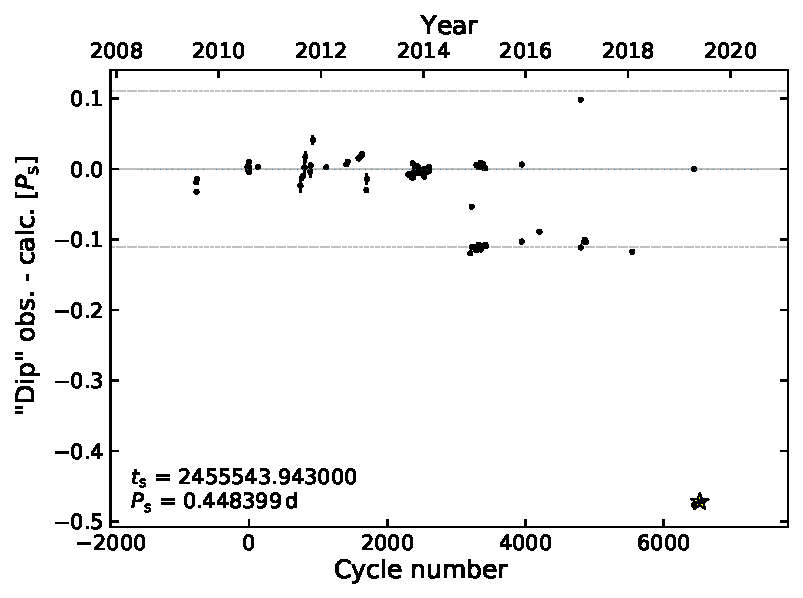
\includegraphics[width=0.45\textwidth]{f4.pdf}
	\end{center}
	\vspace{-0.7cm}
	\caption{ {\bf Scene used for blend analysis.}
		{\it Top:} Mean TESS image of \ptfo\ over Sector~6, with a
		log-stretch.  The position of \ptfo\ is shown with a yellow
		star.  Neighbors with $T<17$ are shown with orange crosses.  The
		apertures used to measure the background and target star flux are
		shown with \texttt{X} and \texttt{/} hatches, respectively.
		{\it Bottom:} Digitized Sky Survey $R$-band image of the same
		field, with a linear stretch. The circles show apertures of radii
		1, 1.5, and 2.25 pixels used in part of our blend analysis.  The
		pixel level TESS data show that ``Star A''  does not contribute
		variability at either of the two observed periods (see
		Section~\ref{subsec:blend}).
		\label{fig:scene}
	}
\end{figure}


The TESS pixels are $\approx21$'' per side, and so before making an
interptations, we need to consider whether light from neighboring
stars could have affected the photometry.  The scene is shown in
Figure~\ref{fig:scene}.  The pixels used to measure the background
level in the SPOC lightcuirve are indicated with an `\texttt{X}'
hatch, and the pixels used in the final lightcurve aperture are shown
with the `\texttt{/}' hatch.

The target star, \ptfo\ (TIC 264461976), has a $T$-band magnitude
of 14.0, and its position is shown with a star.  The other (unlabeled)
star inside the target aperture, TIC 264461979, has $T=16.8$ and so
cannot contribute a signal with relative amplitude 10\%.  The only
neighbor that is sufficiently close and bright that its light might
contaminate the target star is TIC 264461980, with $T=14.8$, which we
denote ``Star A''.  Star A is 23.6'' NW of our target, and based on
the magnitude difference could contribute up to 48\% the flux of our
target star, \ptfo.  

Because \ptfo\ has previously been identified to have periodicity
consistent with our measurement of $P_{\rm s}$, our main concern
regarding blending is the degree to which we can be certain that the
long-period signal at $P_{\rm \ell}$ also originates from \ptfo.
We took two approaches towards determining the source of the
long-period signal.

First, we examined the CDIPS full frame image lightcurves of the
target, which are available on MAST \citep{bouma_cluster_2019}.  The
maximal peak-to-peak beat amplitude is consistently $\approx$10\%
across apertures of radii 1, 1.5, and 2.25 pixels.  If Star A were the
source of the long-period variability, we would expect the peak
variability amplitude to be smallest in the 1 pixel aperture, based on
the separation of the sources (Figure~\ref{fig:scene}, bottom).  From
this test alone, it seems unlikely that Star A is the source of the
long-period signal.

Second, we examined the lightcurve of each pixel in the scene
individually.  We opted to use the interactive tools implemented in
\texttt{lightkurve} \citep{lightkurve_2018}.  If Star A were the
source of the long-period variability, we would expect the pixels
nearest to Star A to show a sinusoidal signal with amplitude exceeding
$10\%$.  We find no evidence for this being the case.  The pixel
directly below Star A does not clearly show the sinusoidal
variability, and the peak-to-peak variability in that pixel is
$\lesssim 8\%$.  In contrast, the south-easternmost pixel within
\ptfo's aperture (the pixel furthest from Star A that was used in the
optimal aperture) shows the $P_{\rm \ell}$ sinusoidal variability
signal at $\approx 10\%$ amplitude.

As there is no evidence in favor of a blend scenario, we conclude that
both the $P_{\rm s}$ and $P_{\rm \ell}$ signals originate from \ptfo,
at least within the resolution of the Gaia-DR2 source catalog.
However, as we shall see, \ptfo itself could still be a binary.


\section{Gaia Analysis \& Photometric Binarity}
\label{sec:gaia}

% \begin{figure*}[t]
% 	\begin{center}
% 		\leavevmode
% 		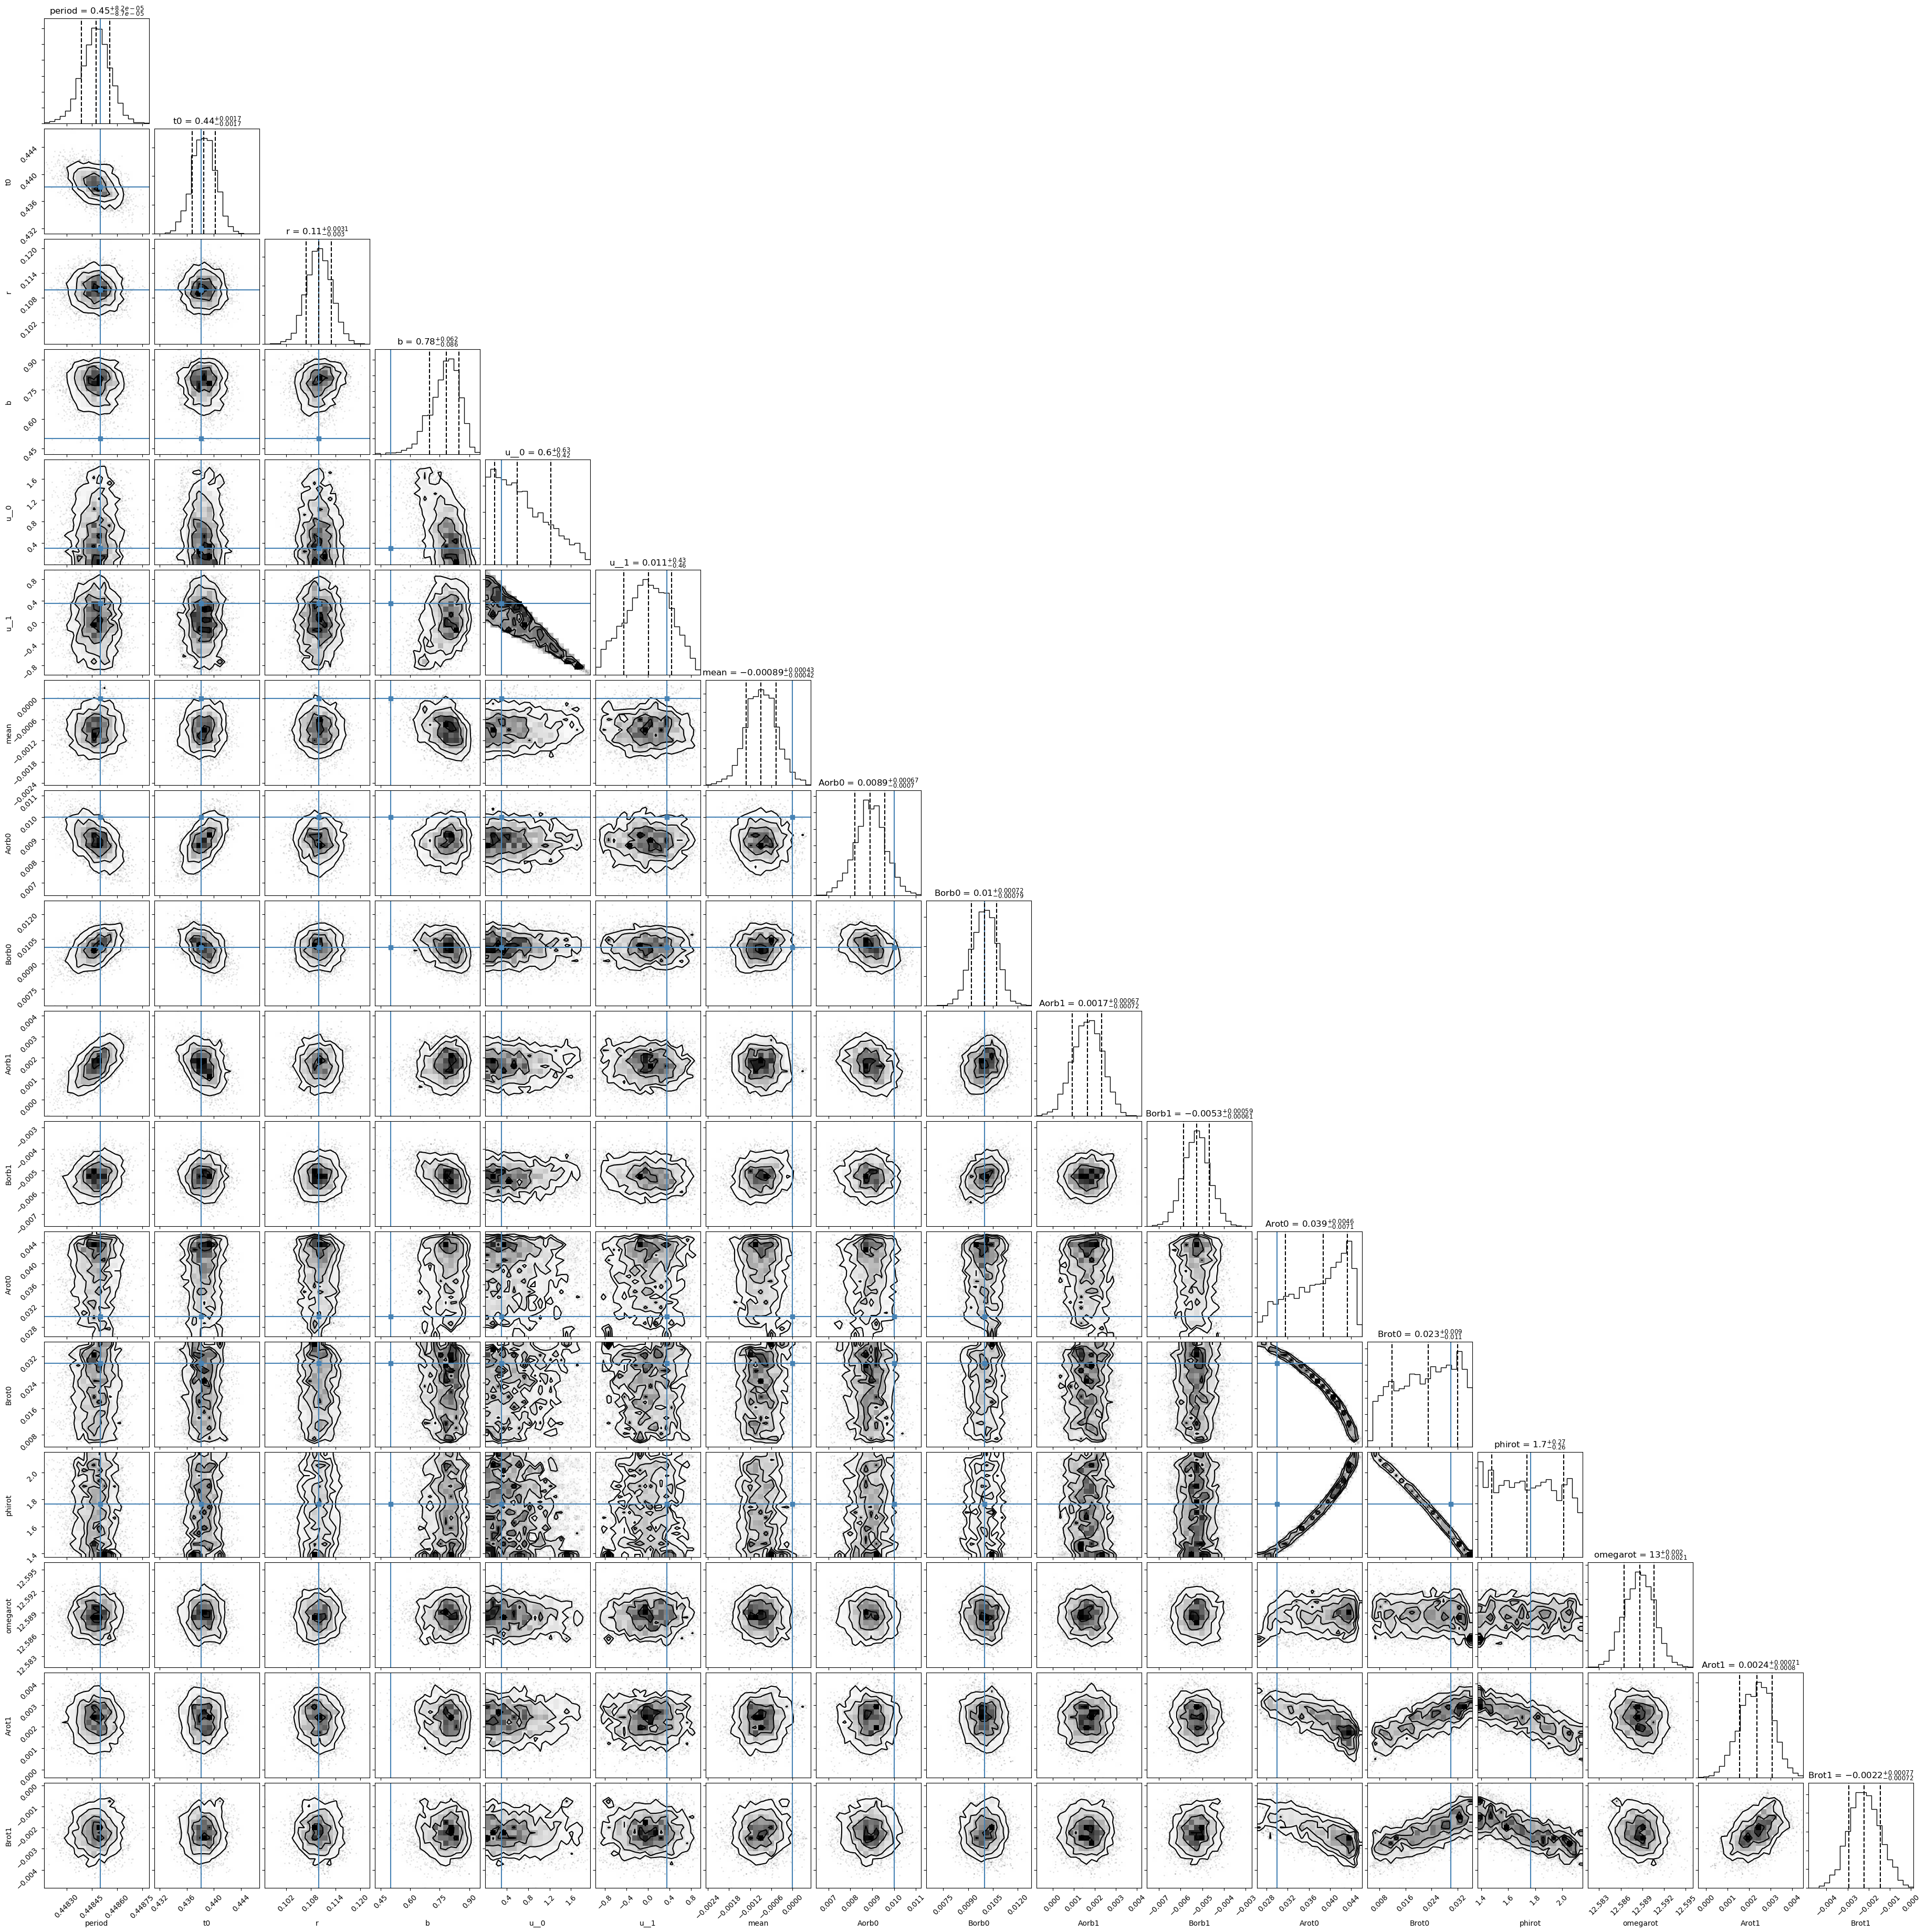
\includegraphics[width=0.9\textwidth]{f6.png}
% 	\end{center}
% 	\vspace{-0.7cm}
% 	\caption{ {\bf Positions, kinematics, and HR diagram of \ptfo.}
%   Members of the 25$\,$Ori-1 subgroup are shown with black circles,
%   and were identified by \citet{kounkel_apogee2_2018} through
%   clustering on Gaia-DR2 and APOGEE data.  The ``neighborhood'' (gray
%   circles) is defined as the group of at most $10^4$ randomly selected
%   non-member stars within 5 standard deviations of the mean right
%   ascension, declination, and parallax.
% 	\label{fig:gaia}
% 	}
% \end{figure*}
\begin{figure*}[t]
	\begin{center}
		\leavevmode
		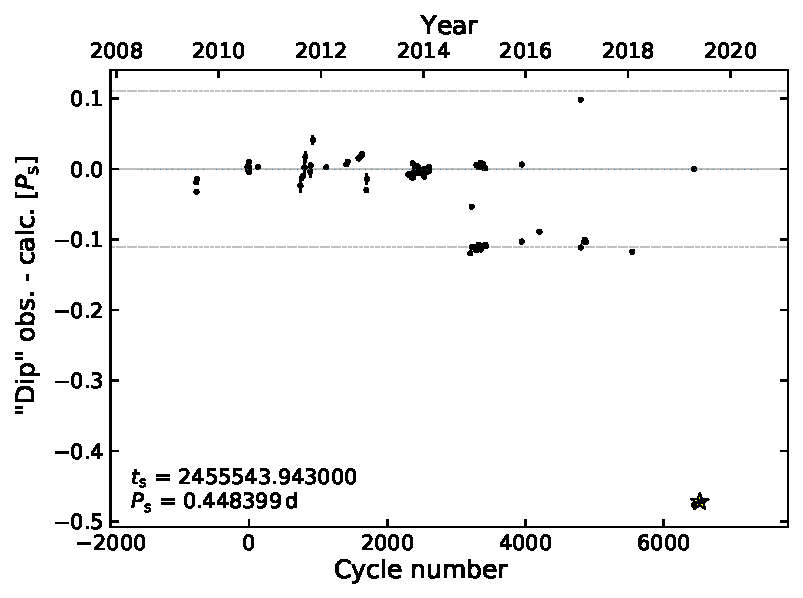
\includegraphics[width=0.8\textwidth]{f5.pdf}
	\end{center}
	\vspace{-0.7cm}
	\caption{ {\bf Hertzsprung-Russell diagram of \ptfo\ and late-type members of 25$\,$Ori-1.}
  Members of the 25$\,$Ori-1 group (black circles) were identified by
  \citet{kounkel_apogee2_2018} through clustering on six-dimensional
  Gaia-DR2 and APOGEE-2 data.  The reference
  ``neighborhood'' (gray circles) is the group of at most $10^4$
  randomly selected non-member stars within 5 standard deviations of
  the mean 25$\,$Ori-1 right ascension, declination, and parallax.
  It contains members of the full Orion complex with a wider spread of ages,
  in addition to field interlopers.
  $G$ is the Gaia broadband, $Bp$ is Gaia blue, $Rp$ is Gaia red, and
  $\omega_{\rm as}$ is the parallax in arcseconds.
  The $x$-axis limits have been set to show only K and M dwarf
  members, to accentuate \ptfo's separation from the
  single-star sequence.
	\label{fig:gaia}
	}
\end{figure*}

%FIXME: summarize existant AO constraints here too
\citet{schmidt_direct_2016}
\citet{lee_evidence_2018}
% \citet{czesla_xray_2019}

To assess the cluster membership and potential
binarity of \ptfo, we needed to identify stars with which it was and was
not coeval.  The simplest way to do this---clustering based on
six-dimensional position and kinematic information---had already been
done by \citet{kounkel_apogee2_2018}.  For simplicity, we considered
the members they identified brighter than $G_{\rm Rp}$ of 16.  This
yielded 149 stars in 25$\,$Ori-1, mostly M dwarfs.
\citet{kounkel_apogee2_2018} identified seven other smaller
groups in the Orion complex near the Be star 25$\,$Ori. These groups
received higher numbers, {\it e.g.}, 25$\,$Ori-2.

To define a set of non-member stars that nonetheless had comparable selection
functions, we defined a reference ``neighborhood'' as the group of at
most $10^4$ randomly selected non-member stars within 5 standard
deviations of the mean 25$\,$Ori-1 right ascension, declination, and
parallax.  We queried these stars using the \texttt{astroquery}
package, which provides a convenient interface to the Gaia archive
(CITE, CITE).  This yielded 1{,}819 neighbors.  While some of
these stars may indeed be members of the Orion complex, or even of
25$\,$Ori-1, enforcing this cut on positions and parallaxes ensures
that we are querying stars with comparable amounts of interstellar
reddening.

We examined the resulting five-dimensional right ascension,
declination, proper motions, and parallaxes.  The first point we noted
was that 25$\,$Ori-1 was a clearly defined over-density in each
dimension, so the cluster exists, and is different from the
neighborhood.  \ptfo\ was also clearly a member in each of these
projected dimensions.

Given our detection of two separate signals, whether
\ptfo\ could be a photometric binary was of great interest.
Figure~\ref{fig:gaia} shows the HR diagram from which we assessed
this issue.
The diagram shows that \ptfo\ is $\approx$0.8 magnitudes brighter than the average
25$\,$Ori-1 star of the same color.
In other words, it is about twice as bright.
It also seems to be on the photometric binary track of the cluster, which has a few other stars.

The implication is that either 
{\it (i)} \ptfo\ is notably younger than the kinematically identical cluster members, or
{\it (ii)} \ptfo\ is a photometric binary.
Given the independent presence of two resolved signals,
we favor the interpretation that \ptfo\ is a binary star system.


\section{Discussion}
\label{sec:discussion}

\subsection{Long period sinusoid}

The standard interpretation of sinusoidal modulations for a pre-main-sequence M
dwarf is that we are observing a stellar rotation period of 11.96 hours.  This
is the dominant signal in the system with 10\% amplitude, and there is no
evidence to suggest that this signal has any other origin.

The discovery study by \citet{van_eyken_ptf_2012} saw the same signal ({\it
e.g.}, their Figure~7), but identified its alias as a periodogram peak at
$0.9985 \pm 0.0061\,$days. They ascribed it to their observing cadence, because
of its close correspondence to the sidereal day.  While the TESS data can show
significant reflected light from the Earth \citep[{\it
e.g.},][]{luger_tess_2019}, our pixel-level analysis showed that the signal is
specific to only pixels near \ptfo, and no other pixels.  We therefore conclude
that the signal is not a systematic.

We are not the first to reach the conclusion that the long period sinusoidal
modulation is astrophysical.  A follow-up study by
\citet{koen_multicolour_2015} identified the same modes and aliases as
\citet{van_eyken_ptf_2012}, but argued that the $0.50\,{\rm d}$ signal was
astrophysical.  Using archival photometry and photometry from the YETI global
telescope network, \citet{raetz_yeti_2016} eventually came to the conclusion
that the that the $0.50\,{\rm d}$ signal was indeed from stellar rotation.  The
TESS data strongly support this conclusion.



\subsection{Short period dip}
The dip lasts about 45 minutes, and seems to re-occur every 10.74
hours
(Figures~\ref{fig:splitsignal},~\ref{fig:splitsignalii},~\ref{fig:phasefold}).
The dip duration is roughly the same as that observed by previous
investigators \citep{van_eyken_ptf_2012,yu_tests_2015}
The dip depth is comparable to what has been observed in red visual
bands...
%TODO: and how does it compare to IR? bigger or smaller? cite relevant
%studies.


\begin{figure}[t]
	\begin{center}
		\leavevmode
		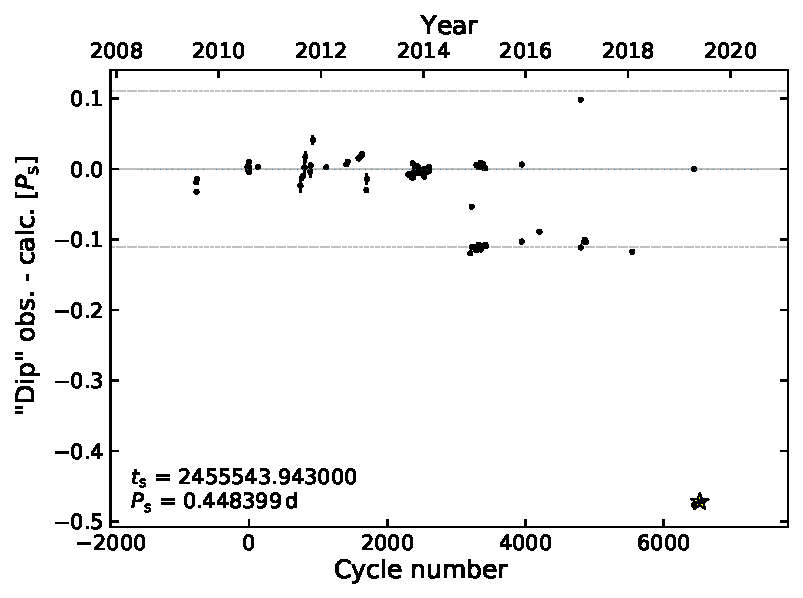
\includegraphics[width=0.5\textwidth]{f6.pdf}
	\end{center}
	\vspace{-0.7cm}
	\caption{
		{\bf Timing residuals for \ptfob\ from a decade of monitoring.}
		Black points are times of ``dips'', minus the indicated linear
		ephemeris.  The $y$-axis is given in units of phase for the
		short-period signal.  The star shows the binned TESS ephemeris.
		``Dips'' have been observed by \citet{van_eyken_ptf_2012},
		\citet{ciardi_followup_2015}, \citet{yu_tests_2015},
		\citet{raetz_yeti_2016}, \citet{onitsuka_multicolor_2017}, and
		\citet{tanimoto_evidence_2020}.  Certain dips ({\it e.g.}, the one
		at phase 0 in mid-2019) are consistent with noise, and were likely
		reported because something was {\it expected}, rather than
		convincingly {\it observed}.  Horizontal dashed lines are drawn at
		$\pm (P_{\rm \ell} - P_{\rm s})/P_{\rm s}$, highlighting a
    possible observational bias.  The orbital phase observed by TESS
    is consistent with that of \citet{tanimoto_evidence_2020}, and
    quite different from the original phase.
		\label{fig:o_minus_c}
	}
\end{figure}

\paragraph{Epoch}
The TESS dip does not phase up where it is supposed to...
Figure~\ref{fig:o_minus_c}

\subsection{Short period out-of-dip modulation}
If there were a giant planet transiting \ptfo, it would tidally
distort the host star, and cause ellipsoidal photometric modulations.
The amplitude of the ellipsoidal distortion for a $1\,M_{\rm Jup}$
companion would be about 1400$\,$ppm
\citep{shporer_astrophysics_2017}.  This is significantly larger than
the typical ellipsopidal modulation induced by close-in giant planets
because the host star is puffy, and still on the pre-main-sequence.
For our estimate, we assumed $R_\star = 1.39 R_\odot$, and $M_\star =
0.39 M_\odot$ \citep{van_eyken_ptf_2012}. 

Our preferred model does detect a significant ellipsoidal signal,
parametrized as the ``$B_1$'' component.  The amplitude of the signal
is $0.53 \pm 0.06\%$.  Interpreted as being caused by a planet, it
would imply a minimum planet mass $M_{\rm p} \sin i$ of $3.8\,M_{\rm
Jup}$.




\section{Physical Interpretation}

%FIXME: the PTFO lightcurve looks so much worse! Why is it less dense??
\begin{figure*}[hbtp]
	\begin{center}
		\leavevmode
		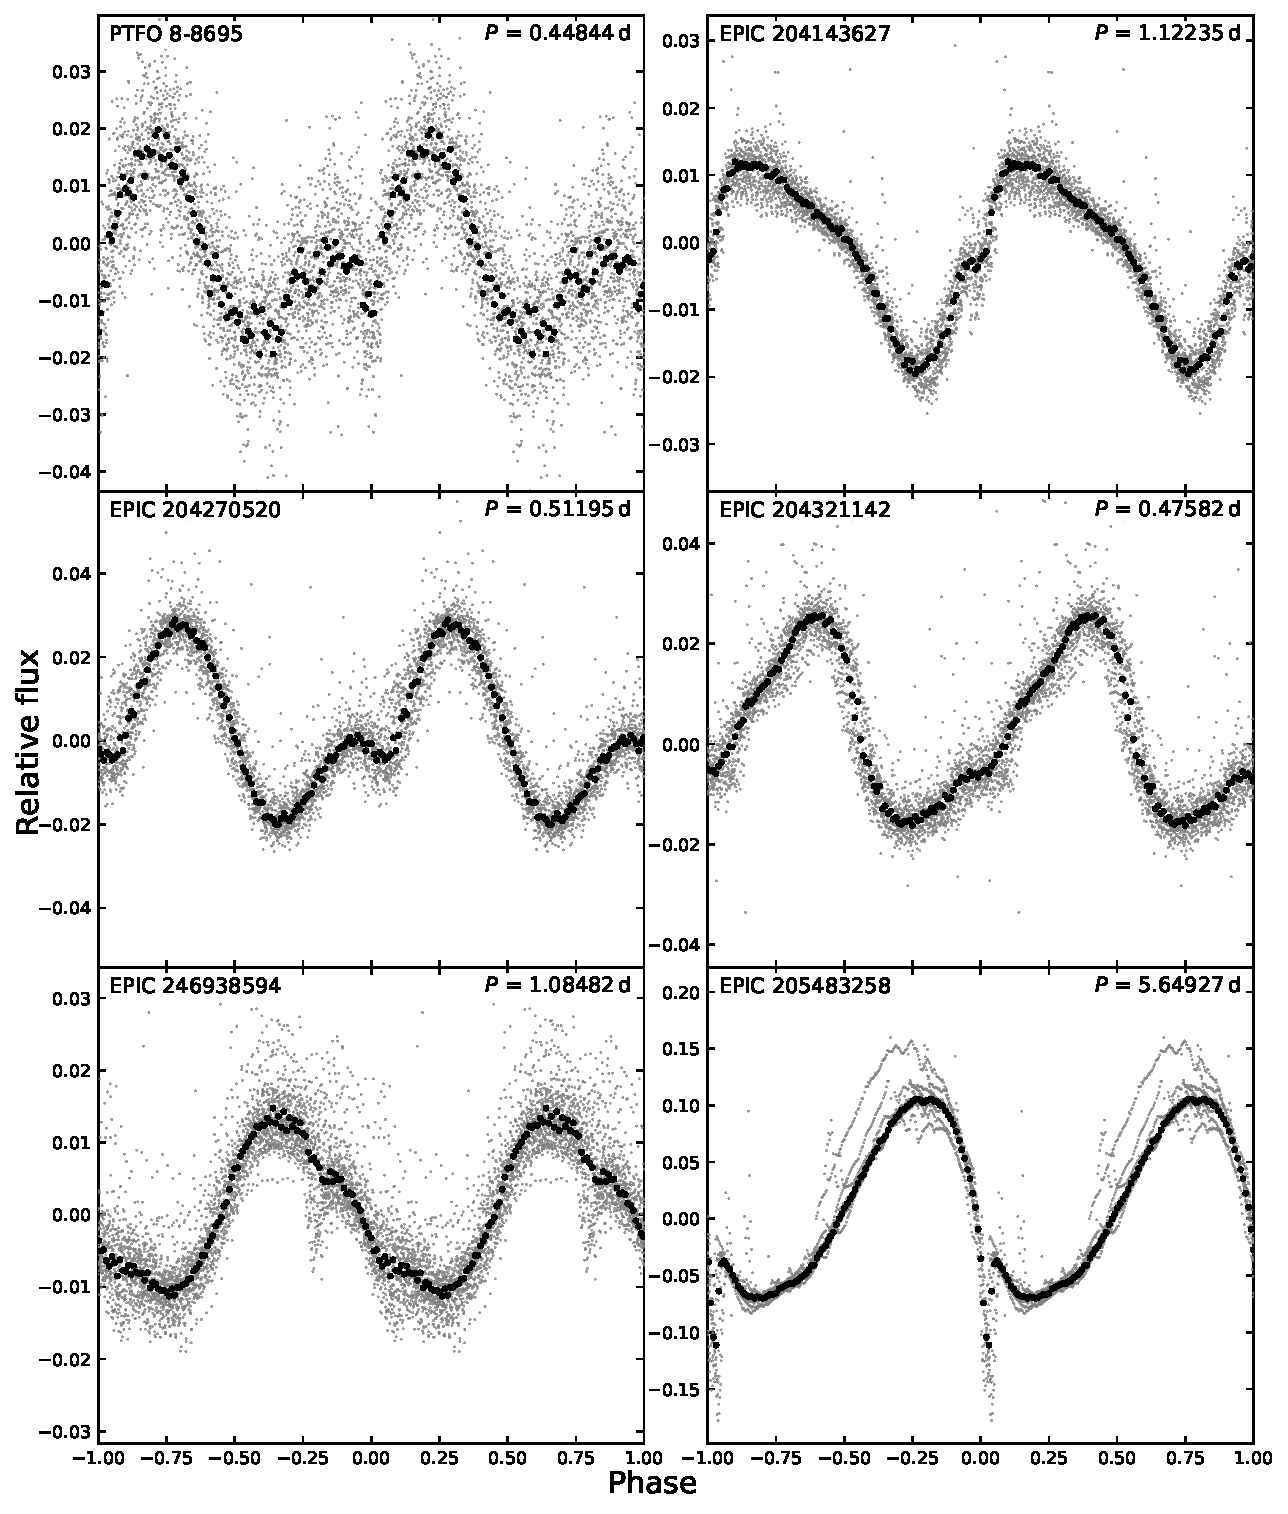
\includegraphics[width=1\textwidth]{f7.pdf}
	\end{center}
	\vspace{-0.7cm}
  \caption{ {\bf \ptfo\ and its brethren.}
  	Five transient and persistent flux dip stars, selected based on their visual similarity to the short-period signal in \ptfo, are as follows.
  	EPIC 204143627, 1.1250d, dips change depth too
  	EPIC 204321142  Usco flux dip, 0.476d
  	EPIC 204270520  USco flux dip, 0.512d
  	% EPIC 205046529B, 1.8358d, indicates dips can be at weird phases too
  	RIK-210 = EPIC 205483258
 	EPIC 204787516  USco flux dip or possible? EB, 0.487d
 	We found these objects through studies by \citet{stauffer_orbiting_2017}, \citet{david_transient_2017}, and \citet{rebull_usco_2018}.
		\label{fig:brethren}
	}
\end{figure*}

cp ../results/brethren/brethren.pdf f7.pdf

Given the evidence, we believe that PTFO$\,$8-8695 is a binary M dwarf
in which one star shows the ``long'' rotation signal, and the other is
showing ``transient dipping'' that has also been observed in other
young M dwarfs. 

Many other young M-dwarf photometric binaries
have been observed in {\it e.g.,} Upper Sco and the Pleiades to show
multiple periods \citep{rebull_usco_2018,stauffer_rotevol_2018}.
Typically, the periods are both rotational modulation.

However, occasionally one or both periods can be ``scallop-shell''
variability, {\it e.g.}, EPIC 203956650 in $\rho$Oph
\citep{rebull_usco_2018}.




There are 

The gas in the disks is gone (CITE).
The upper limits on the SED from \citet{yu_tests_2015} imply X, Y, Z.
The stars are therefore presumably no longer ``magnetically locked''
to their disks.
This is consistent with the $\approx$half-day periodicities of both
signals.
In the broader context of rapidly rotating young M-dwarfs, ``magnetic
locking'' causes classical disked T-Tauri stars tend to rotate more
{\it slowly}, and almost none have periods less than two days
\citep[{\it e.g.},][]{rebull_rotation_2020}.

The main physical question is what is causing the ``transient
dipping''. This is an unsolved problem not only for \ptfo\ but also
for an entire class of young rapidly rotating M-dwarfs



The roughly half-day periods of both signals imply that 






\section{Conclusions}
\label{sec:conclusions}

\ptfo\ was previously thought to potentially host a hot Jupiter.
The TESS lightcurve of \ptfo\ showed a number of new features,
many of which seem to disfavor the hot Jupiter interpretatation.
The TESS data showed two key pieces of evidence.
\begin{enumerate}
  \item {\it Two periodic signals.} The ``long'' signal is a 10\%
      peak-to-peak sinusoidal modulation repeating every 11.96 hours.
      The ``short'' signal is a 4\% peak-to-peak complex modulation
      repeating every 10.74 hours. It is composed of a dip, plus at
      least two harmonics. The signals beat, and therefore cannot be
      an artifact linked to data processing.
  \item {\it A dip at the wrong orbital phase.} The clearest dip in
    the ``short'' signal was consistent with recent observations by
    \citet{tanimoto_evidence_2020}, and differed from the discovery
    epoch by 5.14 hours.
\end{enumerate}

The physical mechanism responsible for all these features remains a
matter of speculation.
With that said, the TESS data support new arguments against the planetary
interpretation of \ptfo.
First, if the long signal is caused by starspot modulation, and the
short signal by a transiting planet, what causes the additional
complex modulations seen at the short, ``orbital'', period?

Similarly, if the planet truly orbits every 10.74 hours, while the
star's equator spins every 11.96 hours, the situation is clearly
Darwin unstable. 



  Given the available evidence,
  PTFO$\,$8-8695 seems consistent with the
  ``transient dipping'' phenomenology observed in many young M dwarfs.
  It seems rather unlikely to be a planet.



%%%%%%%%%%%%%%%%%%%%%%%%%%%%%%%%%%%%%%%%%%%%%%%%%%%%%%%%%%%%%%%%%%%%%%%%%%%%%%%

% \acknowledgements
% %
% This paper includes data collected by the TESS mission, which are
% publicly available from the Mikulski Archive for Space Telescopes
% (MAST).
% %
% Funding for the TESS mission is provided by NASA's Science Mission
% directorate.
% %
% This work made use of NASA's Astrophysics Data System Bibliographic
% Services.
% %
% Based on observations obtained at the Gemini Observatory, which is
% operated by the Association of Universities for Research in Astronomy,
% Inc., under a cooperative agreement with the NSF on behalf of the
% Gemini partnership: the National Science Foundation (United States),
% National Research Council (Canada), CONICYT (Chile), Ministerio de
% Ciencia, Tecnolog\'{i}a e Innovaci\'{o}n Productiva (Argentina),
% Minist\'{e}rio da Ci\^{e}ncia, Tecnologia e Inova\c{c}\~{a}o (Brazil),
% and Korea Astronomy and Space Science Institute (Republic of Korea).
% %
% Observations in the paper made use of the High-Resolution Imaging
% instrument Zorro at Gemini-South. Zorro was funded by the NASA
% Exoplanet Exploration Program and built at the NASA Ames Research
% Center by Steve B. Howell, Nic Scott, Elliott P. Horch, and Emmett
% Quigley.
% %
% This research has made use of the VizieR catalogue access tool, CDS,
% Strasbourg, France. The original description of the VizieR service was
% published in A\&AS 143, 23.
% %
% This work has made use of data from the European Space Agency (ESA)
% mission {\it Gaia} (\url{https://www.cosmos.esa.int/gaia}), processed
% by the {\it Gaia} Data Processing and Analysis Consortium (DPAC,
% \url{https://www.cosmos.esa.int/web/gaia/dpac/consortium}). Funding
% for the DPAC has been provided by national institutions, in particular
% the institutions participating in the {\it Gaia} Multilateral
% Agreement.
%
% (Some of) The data presented herein were obtained at the W. M. Keck
% Observatory, which is operated as a scientific partnership among the
% California Institute of Technology, the University of California and
% the National Aeronautics and Space Administration. The Observatory was
% made possible by the generous financial support of the W. M. Keck
% Foundation.
% The authors wish to recognize and acknowledge the very significant
% cultural role and reverence that the summit of Maunakea has always had
% within the indigenous Hawaiian community.  We are most fortunate to
% have the opportunity to conduct observations from this mountain.
%
% \newline
%

\software{
  \texttt{astrobase} \citep{bhatti_astrobase_2018},
  % \texttt{astroplan} \citep{astroplan2018},
  \texttt{astropy} \citep{astropy_2018},
  \texttt{astroquery} \citep{astroquery_2018},
  % \texttt{BATMAN} \citep{kreidberg_batman_2015},
  \texttt{corner} \citep{corner_2016},
  %\texttt{emcee} \citep{foreman-mackey_emcee_2013},
  \texttt{exoplanet} \citep{exoplanet:agol19}
  \texttt{exoplanet} \citep{exoplanet:exoplanet}, and its
  dependencies \citep{exoplanet:agol19, exoplanet:kipping13, exoplanet:luger18,
  	exoplanet:theano}.
  \texttt{IPython} \citep{perez_2007},
	\texttt{lightkurve} \citep{lightkurve_2018},
  \texttt{matplotlib} \citep{hunter_matplotlib_2007}, 
  \texttt{MESA} \citep{paxton_modules_2011,paxton_modules_2013,paxton_modules_2015}
  \texttt{numpy} \citep{walt_numpy_2011}, 
  \texttt{pandas} \citep{mckinney-proc-scipy-2010},
  \texttt{PyMC3} \citep{salvatier_2016_PyMC3},
  \texttt{radvel} \citep{fulton_radvel_2018},
  % \texttt{scikit-learn} \citep{scikit-learn},
  \texttt{scipy} \citep{jones_scipy_2001}.
}


% \facilities{
% 	{\it Astrometry}:
% 	Gaia \citep{gaia_collaboration_gaia_2016,gaia_collaboration_gaia_2018}.
% 	{\it Imaging}:
% 	Gemini:South~(Zorro; \citealt{scott_nessi_2018}.
% 	{\it Spectroscopy}:
% 	Keck:I~(HIRES; \citealt{vogt_hires_1994}),
% 	Euler1.2m~(CORALIE),
% 	ESO:3.6m~(HARPS; \citealt{mayor_setting_2003}).
% 	{\it Photometry}:
% 	CTIO:1.0m (Y4KCam),
% 	Danish 1.54m Telescope,
% 	El Sauce:0.356m,
% 	Elizabeth 1.0m at SAAO,
% 	Euler1.2m (EulerCam),
% 	Magellan:Baade (MagIC),
% 	Max Planck:2.2m	(GROND; \citealt{greiner_grond7-channel_2008})
% 	NTT,
% 	SOAR (SOI),
% 	TESS \citep{ricker_transiting_2015},
% 	TRAPPIST \citep{jehin_trappist_2011},
% 	VLT:Antu (FORS2).
% }

%
% The following are entries from Table 1 that are not otherwise cited
% in the text
%
% \nocite{wilson_wasp-4b_2008}
% \nocite{gillon_improved_2009}
% \nocite{winn_transit_2009}
% \nocite{hoyer_tramos_2013}
% \nocite{dragomir_terms_2011}
% \nocite{sanchis-ojeda_starspots_2011}
% \nocite{nikolov_wasp-4b_2012}
% \nocite{ranjan_atmospheric_2014}
% \nocite{huitson_gemini_2017}

% \input{WASP-4b_transit_time_table.tex}
% \input{WASP-4b_rv_table.tex}
% \input{model_fit_table.tex}
% \input{rv_model_posterior_table.tex}
% \input{pdot_table.tex}

\clearpage
\startlongtable
\begin{deluxetable*}{lrrrrrrrr}
%
%\tabletypesize{\scriptsize}
%
\tablenum{1}
%
\tablecaption{Model Comparison.}
\label{tab:modelcompare}
%
\tablehead{
\colhead{Description} &
\colhead{$N_{\rm s}$} &
\colhead{$N_{\rm \ell}$} &
\colhead{$N_{\rm data}$} &
\colhead{$N_{\rm param}$} &
\colhead{$\chi^2$} &
\colhead{$\chi_{\rm red}^2$} &
\colhead{BIC} &
\colhead{$\Delta$BIC}
}
% pasted from
% /Users/luke/Dropbox/proj/billy/results/PTFO_8-8695_results/20200413_v0/bic_table_data.tex
\startdata
Favored    & 2 &  2 &   2585 &      17 &  3523.6 &     1.372 &  3657.2 &    0.0 \\
\hline
Somewhat favored & 2 &  3 &   2585 &      19 &  3512.7 &     1.369 &  3662.0 &    4.8 \\
\hline
Disfavored        & 3 &  2 &   2585 &      19 &  3543.1 &     1.381 &  3692.4 &   35.2 \\
---        & 3 &  3 &   2585 &      21 &  3536.8 &     1.379 &  3701.9 &   44.6 \\
---        & 1 &  2 &   2585 &      15 &  3680.0 &     1.432 &  3797.9 &  140.7 \\
---        & 1 &  3 &   2585 &      17 &  3670.2 &     1.429 &  3803.8 &  146.6 \\
---        & 2 &  1 &   2585 &      15 &  3700.9 &     1.440 &  3818.8 &  161.6 \\
---        & 3 &  1 &   2585 &      17 &  3710.2 &     1.445 &  3843.7 &  186.5 \\
---        & 1 &  1 &   2585 &      13 &  3872.7 &     1.506 &  3974.8 &  317.6 \\
\enddata
%
\tablecomments{
	$N_{\rm s}$ and $N_{\rm \ell}$ are the number of harmonics at the short and long periods, respectively.
	$N_{\rm data}$ is the number of fitted flux measurements.
	$N_{\rm param}$ is the number of free parameters in the model.
	The Bayesian information criterion (BIC) and the difference from the maximum $\Delta {\rm BIC}$ are also listed.
}
\vspace{-1cm}
\end{deluxetable*}

% Table of best fit parameters
\startlongtable
\begin{deluxetable*}{llrrrr}
%
\tablecaption{ Best-fit model priors and posteriors. }
\label{tab:posterior}
%
%\tabletypesize{\scriptsize}
%
\tablenum{2}
%
\tablehead{
  \colhead{Param.} & 
  \colhead{Prior} & 
  \colhead{Mean} & 
  \colhead{Std{.} Dev.} &
  \colhead{3\%} &
  \colhead{97\%}
}
% /Users/luke/Dropbox/proj/billy/results/PTFO_8-8695_results/20200413_v0/posterior_table_clean.tex
\startdata
$P_{\rm s}$ & $\mathcal{N}(0.4485; 0.0010)$ & 0.4484732 & 0.0000857 & 0.4483170 & 0.4486367 \\
$t_{\rm s}^{(1)}$ & $\mathcal{N}(0.438096; 0.0020)$ & 0.4384733 & 0.0017440 & 0.4349337 & 0.4415021 \\
$R_{\rm p}/R_\star$ & $\mathcal{N}(0.1100; 0.0033)$ & 0.11 & 0.00308 & 0.10452 & 0.11599 \\
$b$ & $\mathcal{U}(0; 1+R_{\mathrm{p}}/R_\star)$ & 0.7736 & 0.0756 & 0.6346 & 0.8993 \\
$u_1$ & (2) & 0.683 & 0.477 & 0.001 & 1.546 \\
$u_2$ & (2) & 0.004 & 0.417 & -0.793 & 0.727 \\
Mean & $\mathcal{U}(-0.01; 0.01)$ & -0.000885 & 0.000440 & -0.001745 & -0.000088 \\
$\omega_{\rm s}$ & $2\pi/P_{\mathrm{s}}$ & 14.01017 & 0.00268 & 14.00506 & 14.01505 \\
$A_{\mathrm{s},0}$ & $\mathcal{U}(-0.02; 0.02)$ & 0.008903 & 0.000705 & 0.007569 & 0.010277 \\
$B_{\mathrm{s},0}$ & $\mathcal{U}(-0.02; 0.02)$ & 0.009985 & 0.000751 & 0.008504 & 0.011289 \\
$A_{\mathrm{s},1}$ & $\mathcal{U}(-0.02; 0.02)$ & 0.001649 & 0.000696 & 0.000331 & 0.002884 \\
$B_{\mathrm{s},1}$ & $\mathcal{U}(-0.02; 0.02)$ & -0.005267 & 0.000606 & -0.006491 & -0.004203 \\
$\phi_{\rm \ell}$ & $\mathcal{U}(1.3721; 2.1575)$ & 1.74324 & 0.22254 & 1.38274 & 2.08874 \\
$\omega_{\rm \ell}$ & $\mathcal{N}(12.6054; 0.1261)$ & 12.588581 & 0.002040 & 12.584940 & 12.592450 \\
$A_{\mathrm{\ell},0}$ & $\mathcal{U}(-0.06; 0.06)$ & 0.037785 & 0.005150 & 0.028728 & 0.045214 \\
$B_{\mathrm{\ell},0}$ & $\mathcal{U}(-0.06; 0.06)$ & 0.022288 & 0.008592 & 0.008066 & 0.0359 \\
$A_{\mathrm{\ell},1}$ & $\mathcal{U}(-0.02; 0.02)$ & 0.002326 & 0.000756 & 0.000857 & 0.003658 \\
$B_{\mathrm{\ell},1}$ & $\mathcal{U}(-0.02; 0.02)$ & -0.002197 & 0.000744 & -0.003512 & -0.000743 \\
\enddata
%\tablenotetext{}{ 240000 links saved}
\tablenotetext{}{
  (1) To convert mean TESS mid-transit time to ${\rm BJD}_{\rm TDB}$, add 2458468.2.
  (2) Quadratic limb-darkening prior from \citet{exoplanet:kipping13}, implemented by \citet{exoplanet:exoplanet}.
}
\vspace{0cm}
\end{deluxetable*}

\clearpage

\bibliographystyle{yahapj}                            
\bibliography{bibliography} 


\listofchanges

\end{document}
